%Dokumentklasse

%draft als option ohne bilder für bessere performance
%\documentclass[a4paper,12pt,]{scrreprt}

%normal mit Bildern
\documentclass[
a4paper,
12pt,
draft=True]
{scrartcl}

%angepasster \today Command
\newcommand{\leadingzero}[1]{\ifnum #1<10 0\the#1\else\the#1\fi}
\newcommand{\todayDE}{\leadingzero{\day}.\leadingzero{\month}.\the\year}

%Section als Chapter
\RedeclareSectionCommand[%
%beforeskip = -1sp plus -1sp minus -1sp,% kleinster negativer Wert, um den Absatzeinzug nach der Überschrift zu verhindern.
afterskip = 1.5 \baselineskip plus -1sp minus 1sp,
font = \Huge,
]{section}

\usepackage[left= 3cm,right = 3cm, bottom = 3cm,top = 3cm]{geometry}
%\usepackage[onehalfspacing]{setspace}

% ============= Packages =============
% Dokumentinformationen
\usepackage[
pdftitle={Praktikum - Umwelttechnik},
pdfsubject={},
pdfauthor={Roman-Luca Zank},
pdfkeywords={},	
%Links nicht einrahmen
hidelinks
]{hyperref}

%nur Text zum prüfen des Umfangs

% Standard Packages
%\usepackage[bottom]{footmisc}
\usepackage[utf8]{inputenc}
\usepackage[ngerman]{babel}

\usepackage[T1]{fontenc}
%\usepackage{helvet}

%\renewcommand{\familydefault}{\sfdefault}

\usepackage{colortbl}
\usepackage{graphicx}
\graphicspath{{img/}}
\usepackage{mhchem}
\usepackage{fancyhdr}
\usepackage{lmodern}
\usepackage[table]{xcolor}
\usepackage{placeins}
\usepackage{booktabs}
\usepackage{caption}
\usepackage[list=true]{subcaption}
\usepackage{longtable}
\usepackage{tikz}
\usepackage{pgfplots}
\pgfplotsset{/pgf/number format/use comma}
\pgfplotsset{grid style={white!90!black}}
\usepackage{lastpage}
%\usepackage{ulem}
\usepackage{mathtools}
\usepackage{adjustbox}
\usetikzlibrary{patterns}
\usepackage{pdfpages}
\usepackage[shortlabels]{enumitem}

%Einheitenpackage
\usepackage{siunitx}  
\sisetup{	locale = DE, 
	per-mode=fraction,
	inter-unit-product=\ensuremath{\cdot},
	detect-weight = true,
	quotient-mode=fraction
}
%neue Einheiten definieren
\DeclareSIUnit\xyz{xyz}	
\DeclareSIUnit\rpm{rpm}	
\DeclareSIUnit\mws{mWS}	
\DeclareSIUnit\degrees{^\circ}	
\DeclareSIUnit\kmeter{\raiseto{3} \meter}	
\DeclareSIUnit\smeter{\raiseto{2} \meter}	

%Automatisch cdot statt *
\DeclareMathSymbol{*}{\mathbin}{symbols}{"01}


%Tabelle
\usepackage{tabularx}
\usepackage{tabulary}

%nur letzte Zeile der Gleichung nummerieren
\makeatletter
\def\Let@{\def\\{\notag\math@cr}}
\makeatother

% zusätzliche Schriftzeichen der American Mathematical Society
\usepackage{amsfonts}
\usepackage{amsmath}

%Abkürzungsverzeichnis
\usepackage{acronym}

%kein Abstand bei neuem Kapitel vom Seitenanfang
%\vspace*{2.3\baselineskip} = ORIGINAL
%\renewcommand*{\chapterheadstartvskip}{\vspace*{.0\baselineskip}}

%nicht einrücken nach Absatz
\setlength{\parindent}{0pt}


\urlstyle{same}

% ============= Kopf- und Fußzeile =============
\pagestyle{fancy}
%
\lhead{}
\chead{}
\rhead{}%\slshape }%\leftmark}
%%
\lfoot{}
\cfoot{}
\rfoot[{\thepage\ of \pageref*{LastPage}}]{Seite \thepage\ von \pageref*{LastPage}}
%%
\renewcommand{\headrulewidth}{0pt}
\renewcommand{\footrulewidth}{0pt}
%\renewcommand{\chapterpagestyle}{fancy}

%Fußnotelinie
%\let\footnoterule

%Fußnote mit Klammer
\renewcommand*{\thefootnote}{(\arabic{footnote})}

%Abb. statt Abbildung
\addto\captionsngerman{%
	\renewcommand{\figurename}{Abb.}%
	\renewcommand{\tablename}{Tab.}%
}

% ============= Package Einstellungen & Sonstiges ============= 
%Besondere Trennungen
%\hyphenation{De-zi-mal-tren-nung}
\usepackage[none]{hyphenat}
\hyphenpenalty=5000
\tolerance=5000
\providecommand\phantomsection{}

\usepackage{mathtools}


% ============= Dokumentbeginn =============

\begin{document}
%Seiten ohne Kopf- und Fußzeile sowie Seitenzahl
\pagestyle{empty}

%\begin{center}
\begin{tabular}{p{\textwidth}}


\begin{center}

\includegraphics[scale=0.75]{logos.jpg}\\
\end{center}


\\

\begin{center}
\LARGE{\textsc{Einführung in die Laborpraktika\\
}}
\end{center}

\\

%\begin{center}
%\large{Fakultät für Muster und Beispiele \\
%der Hochschule Musterhausen \\}
%\end{center}
%
%\\

\begin{center}
\textbf{\Large{Handout mit allgemeinen Hinweisen für \mbox{chemie- und umwelttechnische} Praktika}}
\end{center}


\\
%\begin{center}
%zur Erlangung des akademischen Grades\\
%Bachelor of Engineering
%\end{center}


%\begin{center}
%vorgelegt von
%\end{center}

\begin{center}
	\includegraphics[scale=0.75]{img/versuchsaufbau_1}\\
\end{center}
%Ende

\begin{center}
	Diese Übersicht soll für zukünftige Praktika in Form von Vorschlägen und Wissen eine Unterstützung bieten, um Geräte oder Versuchsstände selbstständig bedienen und aufbauen zu können.
\end{center}


\\ \\

%\begin{center}
%\begin{tabular}{lll}
%\large{\textbf{Protokollführer:}} & & \large{Roman-Luca Zank}\\
%&&\\
%\large{\textbf{Datum der Versuchsdurchführung:}}&& \large{22.10.2020}\\
%&&\\
%\large{\textbf{Abgabedatum:}}&& \large{\todayDE}
%\end{tabular}
%\end{center}

\end{tabular}
\end{center}

\vfill
\large{Merseburg den \todayDE}


%\include{14_danksagungen}

%\include{15_zusammenfassung}

% Beendet eine Seite und erzwingt auf den nachfolgenden Seiten die Ausgabe aller Gleitobjekte (z.B. Abbildungen), die bislang definiert, aber noch nicht ausgegeben wurden. Dieser Befehl fügt, falls nötig, eine leere Seite ein, sodaß die nächste Seite nach den Gleitobjekten eine ungerade Seitennummer hat. 
\cleardoubleoddpage

% Pagestyle für Titelblatt leer
\pagestyle{empty}

%Seite zählen ab
\setcounter{page}{0}

%Titelblatt
\begin{center}
\begin{tabular}{p{\textwidth}}


\begin{center}

\includegraphics[scale=0.75]{logos.jpg}\\
\end{center}


\\

\begin{center}
\LARGE{\textsc{Einführung in die Laborpraktika\\
}}
\end{center}

\\

%\begin{center}
%\large{Fakultät für Muster und Beispiele \\
%der Hochschule Musterhausen \\}
%\end{center}
%
%\\

\begin{center}
\textbf{\Large{Handout mit allgemeinen Hinweisen für \mbox{chemie- und umwelttechnische} Praktika}}
\end{center}


\\
%\begin{center}
%zur Erlangung des akademischen Grades\\
%Bachelor of Engineering
%\end{center}


%\begin{center}
%vorgelegt von
%\end{center}

\begin{center}
	\includegraphics[scale=0.75]{img/versuchsaufbau_1}\\
\end{center}
%Ende

\begin{center}
	Diese Übersicht soll für zukünftige Praktika in Form von Vorschlägen und Wissen eine Unterstützung bieten, um Geräte oder Versuchsstände selbstständig bedienen und aufbauen zu können.
\end{center}


\\ \\

%\begin{center}
%\begin{tabular}{lll}
%\large{\textbf{Protokollführer:}} & & \large{Roman-Luca Zank}\\
%&&\\
%\large{\textbf{Datum der Versuchsdurchführung:}}&& \large{22.10.2020}\\
%&&\\
%\large{\textbf{Abgabedatum:}}&& \large{\todayDE}
%\end{tabular}
%\end{center}

\end{tabular}
\end{center}

\vfill
\large{Merseburg den \todayDE}
 %Protokolle
%\begin{center}
\begin{tabular}{p{\textwidth}}


\begin{center}

\includegraphics[scale=0.75]{img/logos.jpg}\\
\end{center}


\\

\begin{center}
\LARGE{\textsc{
Recherche \\
Rückgewinnung von Ammoniak aus Industrieabwässern\\
}}
\end{center}

%\begin{center}
%\large{Fakultät für Muster und Beispiele \\
%der Hochschule Musterhausen \\}
%\end{center}
%
%\\
 \\
 
\begin{center}
\textbf{\Large{Seminararbeit in Medienrecherche}}
\end{center}

\begin{center}
	\large{im WiSe 2019}
\end{center}
 \\
%\begin{center}
%zur Erlangung des akademischen Grades\\
%Bachelor of Engineering
%\end{center}


\begin{center}
\large{vorgelegt von}
\end{center}
\\


\begin{center}
\Large{\textbf{Roman-Luca Zank}} \\
\end{center}

\begin{center}
3. Semester \\
Chemie- und Umwelttechnik \\
\end{center}


\begin{center}
\begin{tabular}{lll}
	\textbf{E-Mail:} & & romanzank@mail.de\\
	\textbf{Matrikelnummer:} & &25240\\
	\textbf{Adresse:} & &Platz der Bausoldaten 2, Zimmer 224\\
	\textbf{Ort:} & &06217 Merseburg\\
	&& \\
	\textbf{Prüfer:} & & Dr. Frank  Baumann\\
\end{tabular}
\end{center}

\\ \\ \\ \\ \\
\large{Merseburg, \today}

\end{tabular}
\end{center}
 %Seminar-/Abschlussarbeit

% Pagestyle für Rest des Dokuments
\pagestyle{fancy}

%Inhaltsverzeichnis
\tableofcontents
%\thispagestyle{empty}
%\newpage

%Inhalt
%
%Verzeichnis aller Bilder
\label{sec:bilder}
\listoffigures
\addcontentsline{toc}{chapter}{Abbildungsverzeichnis}
\thispagestyle{empty}

%Verzeichnis aller Tabellen
\label{sec:tabellen}
\listoftables
\addcontentsline{toc}{chapter}{Tabellenverzeichnis}
\thispagestyle{empty}



\section{Theoretische Grundlagen}
Um in Seminarräumen, Hörsälen oder Klassenzimmer das Risiko von einer Vireninfektion gering zu halten, ist eine gute Durchlüftung des jeweiligen Raumes nötig. Wie oft gelüftet werden sollte hängt von mehreren Parametern ab, welche sich gerade für Aerosole als kompliziert erweisen. \\
Hierbei werden Modelle für die Tröpfchenbildung, deren Sinkgeschwindigkeit, sowie Effizienz der Masken und ähnliches zurate gezogen. \\
Um dennoch eine sinnvolle Belüftung von Räumlichkeiten zu gewährleisten, können bereits untersuchte Luftparameter wie der CO2-Gehalt in Arbeitsräumen genutzt werden. Für diese Annahme wird davon ausgegangen, dass je mehr CO¬2 sich in der Luft befindet, desto höher ist das Risiko, dass bereits ausgeatmete Luft zusammen mit Aerosolen wieder eingeatmet wird. \\
Über den CO2-Gehalt kann somit eine indirekte Messung an Aerosolen erfolgen und entsprechende Messgeräte wie CO2-Ampeln auf ein Mindestmaß an Lüftung hinweisen.\\
Doch wie lässt sich nun der CO2-Gehalt in einem Raum bestimmen? Welche Kriterien für die maximale Konzentration sollen dabei eingehalten werden? \cite{Hartmann.2020,Simmank.15.08.2020,bghm2020}

\subsection{Die Pettenkofer-Zahl}
Prof. Max Pettenkofer (1818-1901) definierte bereits 1858 eine anzustrebende Obergrenze für den \ce{CO2}-Gehalt in einem Raum von 1000 ppm = 0,10 Vol.\%. Dieser Grenzwert ist auch heute noch als \textsc{Pettenkofer}-Zahl bekannt.
Entstanden aus der Zeit der Industrialisierung und als technische Regel an Arbeitsstätten hinzugezogen, beweist sich auch heute noch die \textsc{Pettenkofer}-Zahl bzw. der \ce{CO2}-Gehalt der Luft, als effektives Maß für die Bewertung der Luftqualität in Innenräumen. 
In der Lüftungsnorm \mbox{DIN 1946 Teil 2} wird ein maximaler Wert von 1500 ppm = 0,15 Vol.\% angegeben.

\subsection{Einflussgrößen für den \ce{CO2}-Gehalt in einem Raum}
Der \ce{CO2}-Gehalt in Räumen hängt von verschiedenen Parametern ab, ähnlich wie der Aerosolgehalt. Untersuchungen des \ce{CO2}-Gehaltes legen jedoch sehr verständliche Annahmen und Messwerte nahe, welche eine gute Durchlüftung zum Niedrighalten des Aerosolgehaltes bestimmen lassen.

\subsubsection*{Aktivität}
Je nachdem welche Aktivitäten die, sich im Raum befindlichen Personen ausüben wird pro Zeiteinheit ein höheres oder niedrigeres Maß an \ce{CO2} freigesetzt. In der folgenden Tabelle 1 findet sich eine Auswahl solcher Volumenströme nach VDI 4300 Blatt 7.

\begin{table}[h!]
	\renewcommand*{\arraystretch}{1.2}
	\centering
	\rowcolors{2}{white}{gray!25}
	\caption{\ce{CO2}- Abgabe einer erwachsenen Person bei verschiedenen körperlichen Aktivitäten (VDI 4300 Blatt 7)}
	\label{tab:aktivitaeten}
		\begin{tabulary}{1.0\textwidth}{C|C}
			\hline
			\textbf{Aktivität} 	& \textbf{$\boldmath \dot{V}_{\ce{CO2}}$ in \si{\liter \per \hour}}\\
			\hline
			Sitzende Tätigkeit 	& 15 - 20 \\
			Leichte Arbeit			& 20 - 40 \\
			Mittelschwere Arbeit & 40 - 70 \\
			Schwere Arbeit 	& 70 - 110\\
			\hline			
		\end{tabulary}
\end{table}
\FloatBarrier
\vspace*{-5mm}
\subsubsection*{Personenzahl}
Auch die Personenanzahl in einem Raum spielt eine wichtige Rolle. Je nachdem wie viele Personen sich in einem Raum befinden, wird die vorhandene Luft unterschiedlich schnell aufgebraucht und mit ausgeatmeter Luft ersetzt bzw. mit Aerosolen versehen.

\subsubsection*{Zeit}
Dieser Punkt versteht sich von selbst, denn je mehr Zeit vergeht, desto mehr Luft wird eingeatmet und desto mehr \ce{CO2} bzw. Aerosole werden ausgeatmet.

\subsubsection*{Raumvolumen}
Je größer der Raum ist, desto mehr Luftkapazitäten sind vorhanden. Je größer der Raum bei gleicher Personenzahl ist, desto geringer ist das Risiko Aerosole einzuatmen.

\subsubsection*{Luftwechselzahl}
Die Luftwechselzahl gibt an wie oft das komplette Raumvolumen innerhalb einer Stunde ausgewechselt wird. Sie ist also ein maßgeblicher Parameter zur Kontrolle des \ce{CO2}-Gehaltes bzw. der Aerosole im Raum. Wie groß die Luftwechselzahl ist hängt dabei unter anderem von der Anzahl geöffneter Türen oder Fenster, sowie Belüftungsanlagen ab.

\begin{table}[h!]
	\renewcommand*{\arraystretch}{1.2}
	\centering
	\rowcolors{2}{white}{gray!25}
	\caption{Lüftungszahlen für verschiedene Fensterlüftungen \cite{Bosy.17.10.2020}}
	\label{tab:lueftungen}
	\begin{tabulary}{1.1\textwidth}{C|C}
		\hline
		\textbf{Zustand} 	& \textbf{$\boldmath n$ in \si{\per \hour}}\\
		\hline
		Fenster zu, Türen zu 												& $> 0,0 \text{ bis } 0,3$\\
		Fenster gekippt (Spaltlüftung)  						& $> 0,3 \text{ bis } 1,5$\\
		Fenster kurzzeitig ganz geöffnet (Stoßlüftung) & $> 0,3 \text{ bis } 4,0$\\
		Fenster ständig ganz geöffnet & $> 9,0 \text{ bis } 15,0$\\
		Gegenüberliegende Fenster und Türen ständig geöffnet (Querlüftung) & $> 40$\\
		\hline			
	\end{tabulary}
\end{table}
\FloatBarrier
	
\begin{figure}[h!]
		\centering
		\begin{minipage}{0.45\textwidth}
			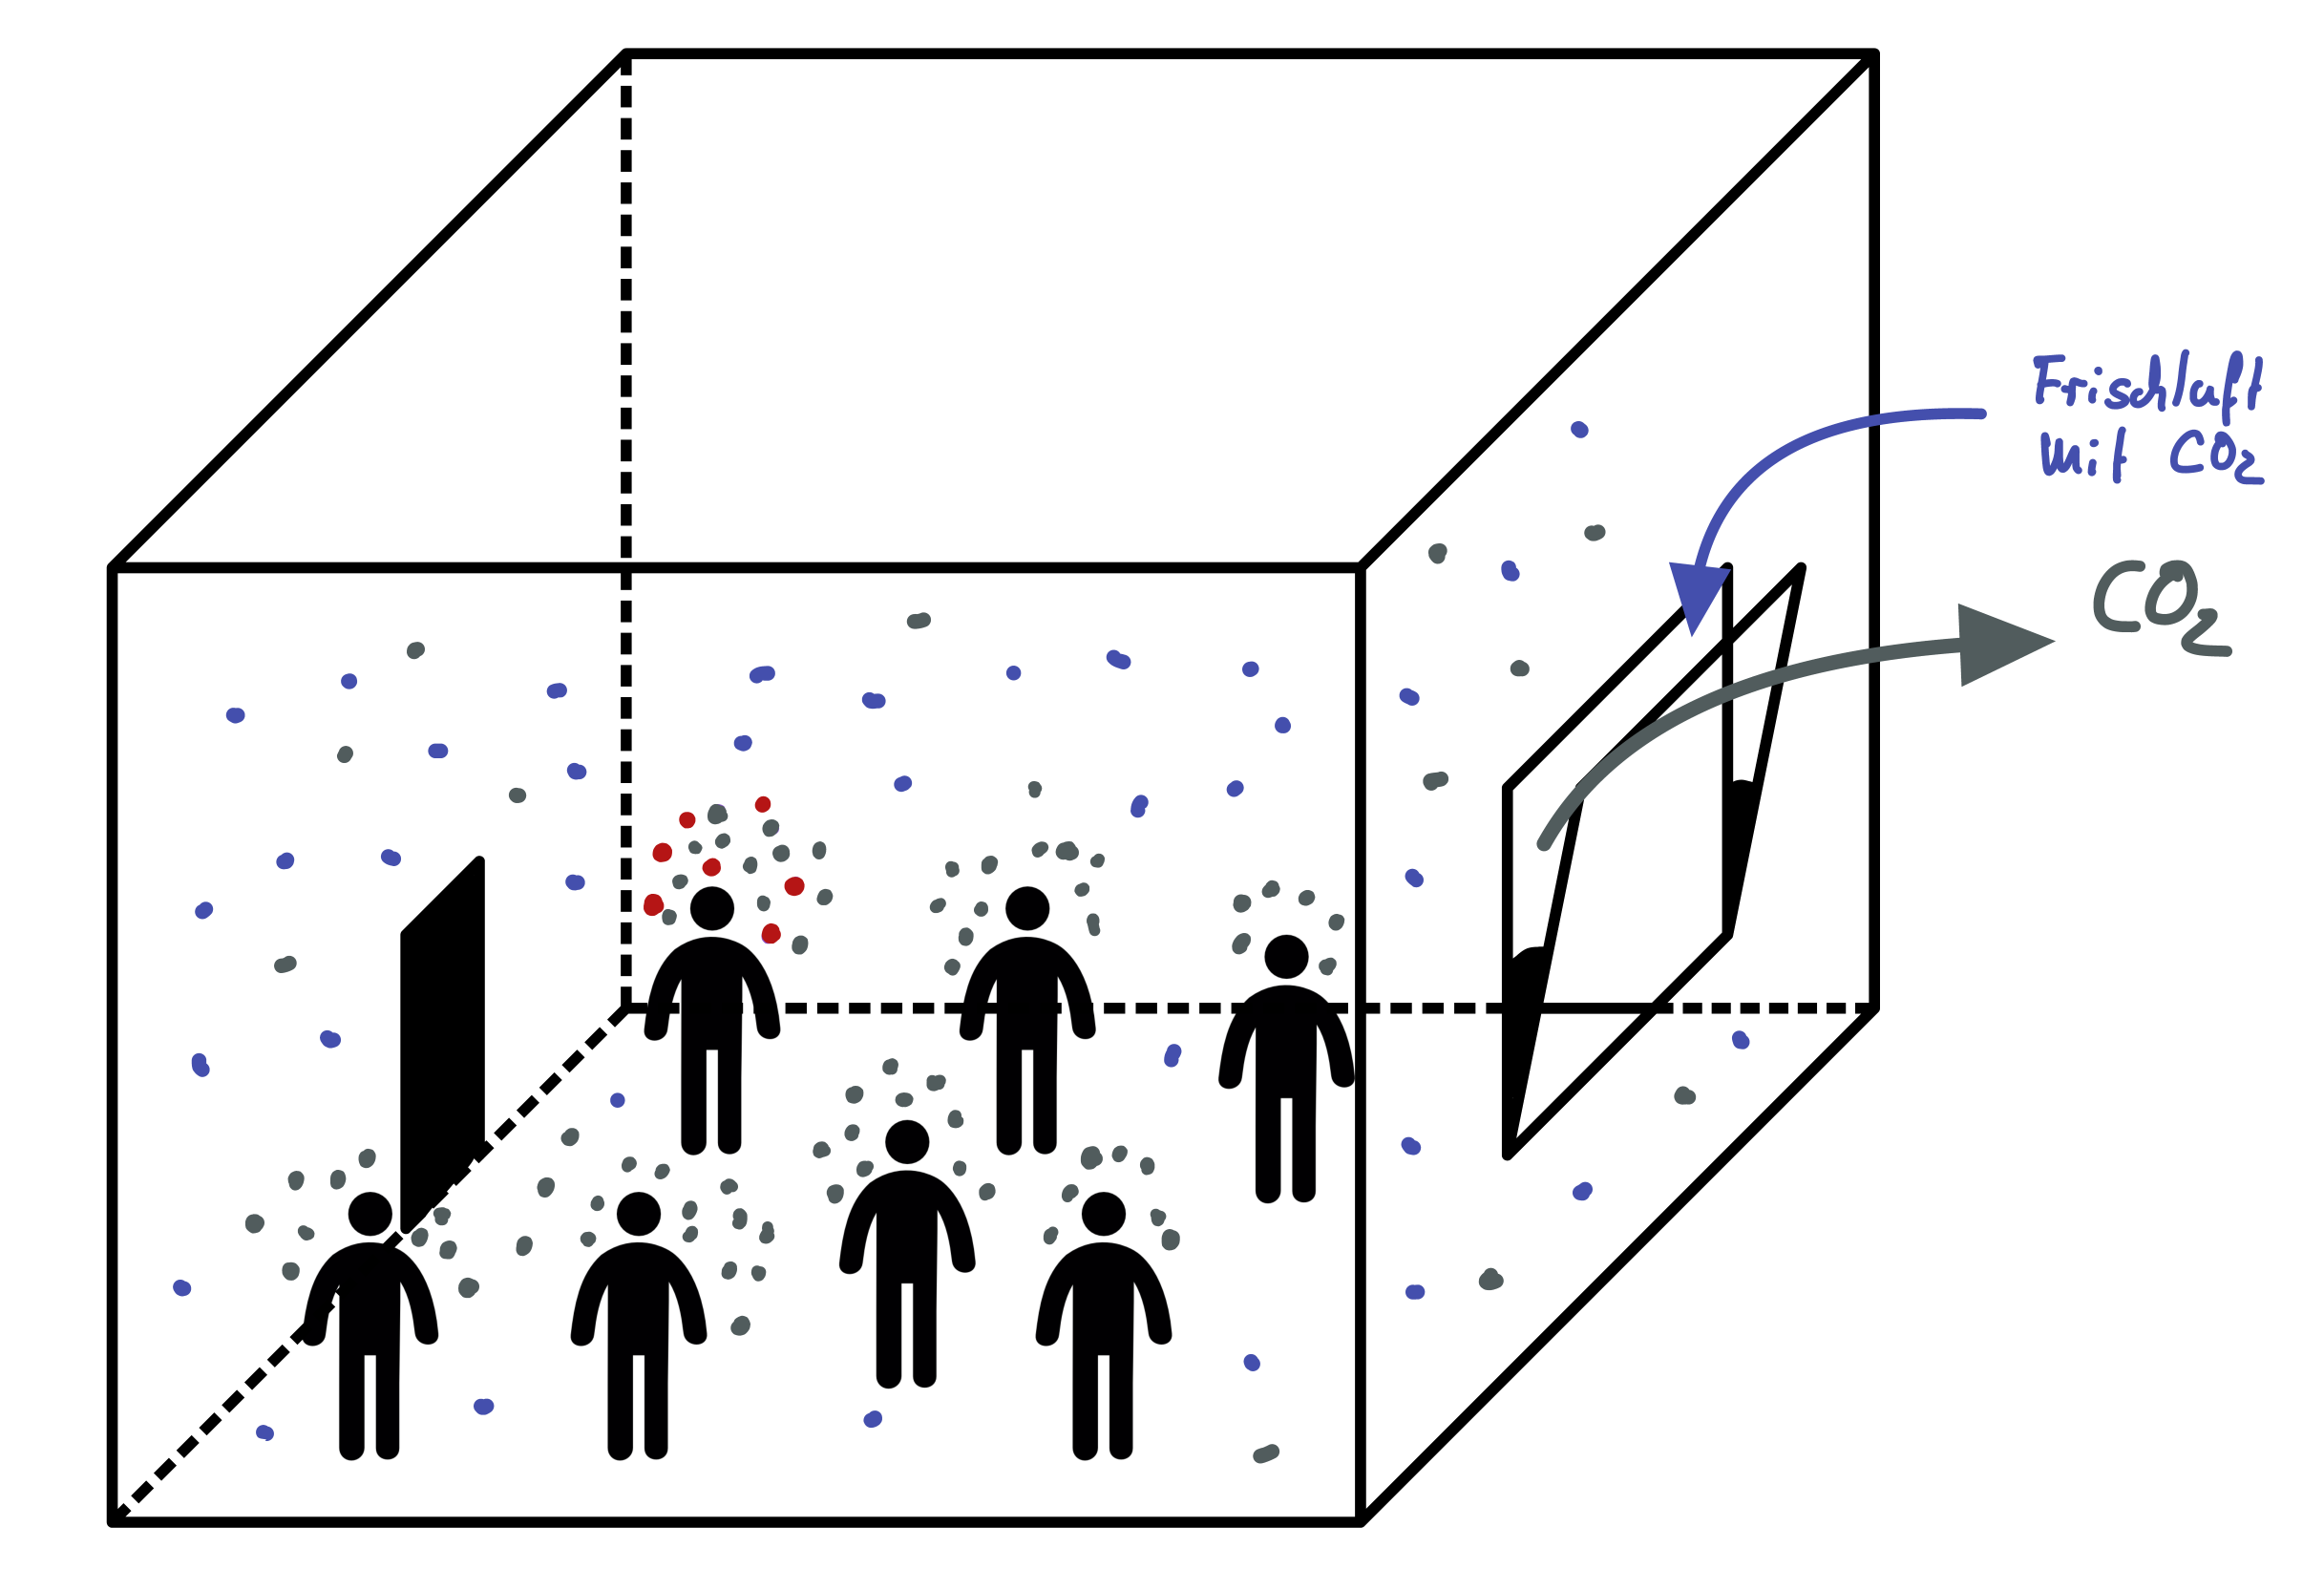
\includegraphics[width=1.\textwidth]{img/spaltluft}
		\end{minipage}
	\begin{minipage}{0.45 \textwidth}
			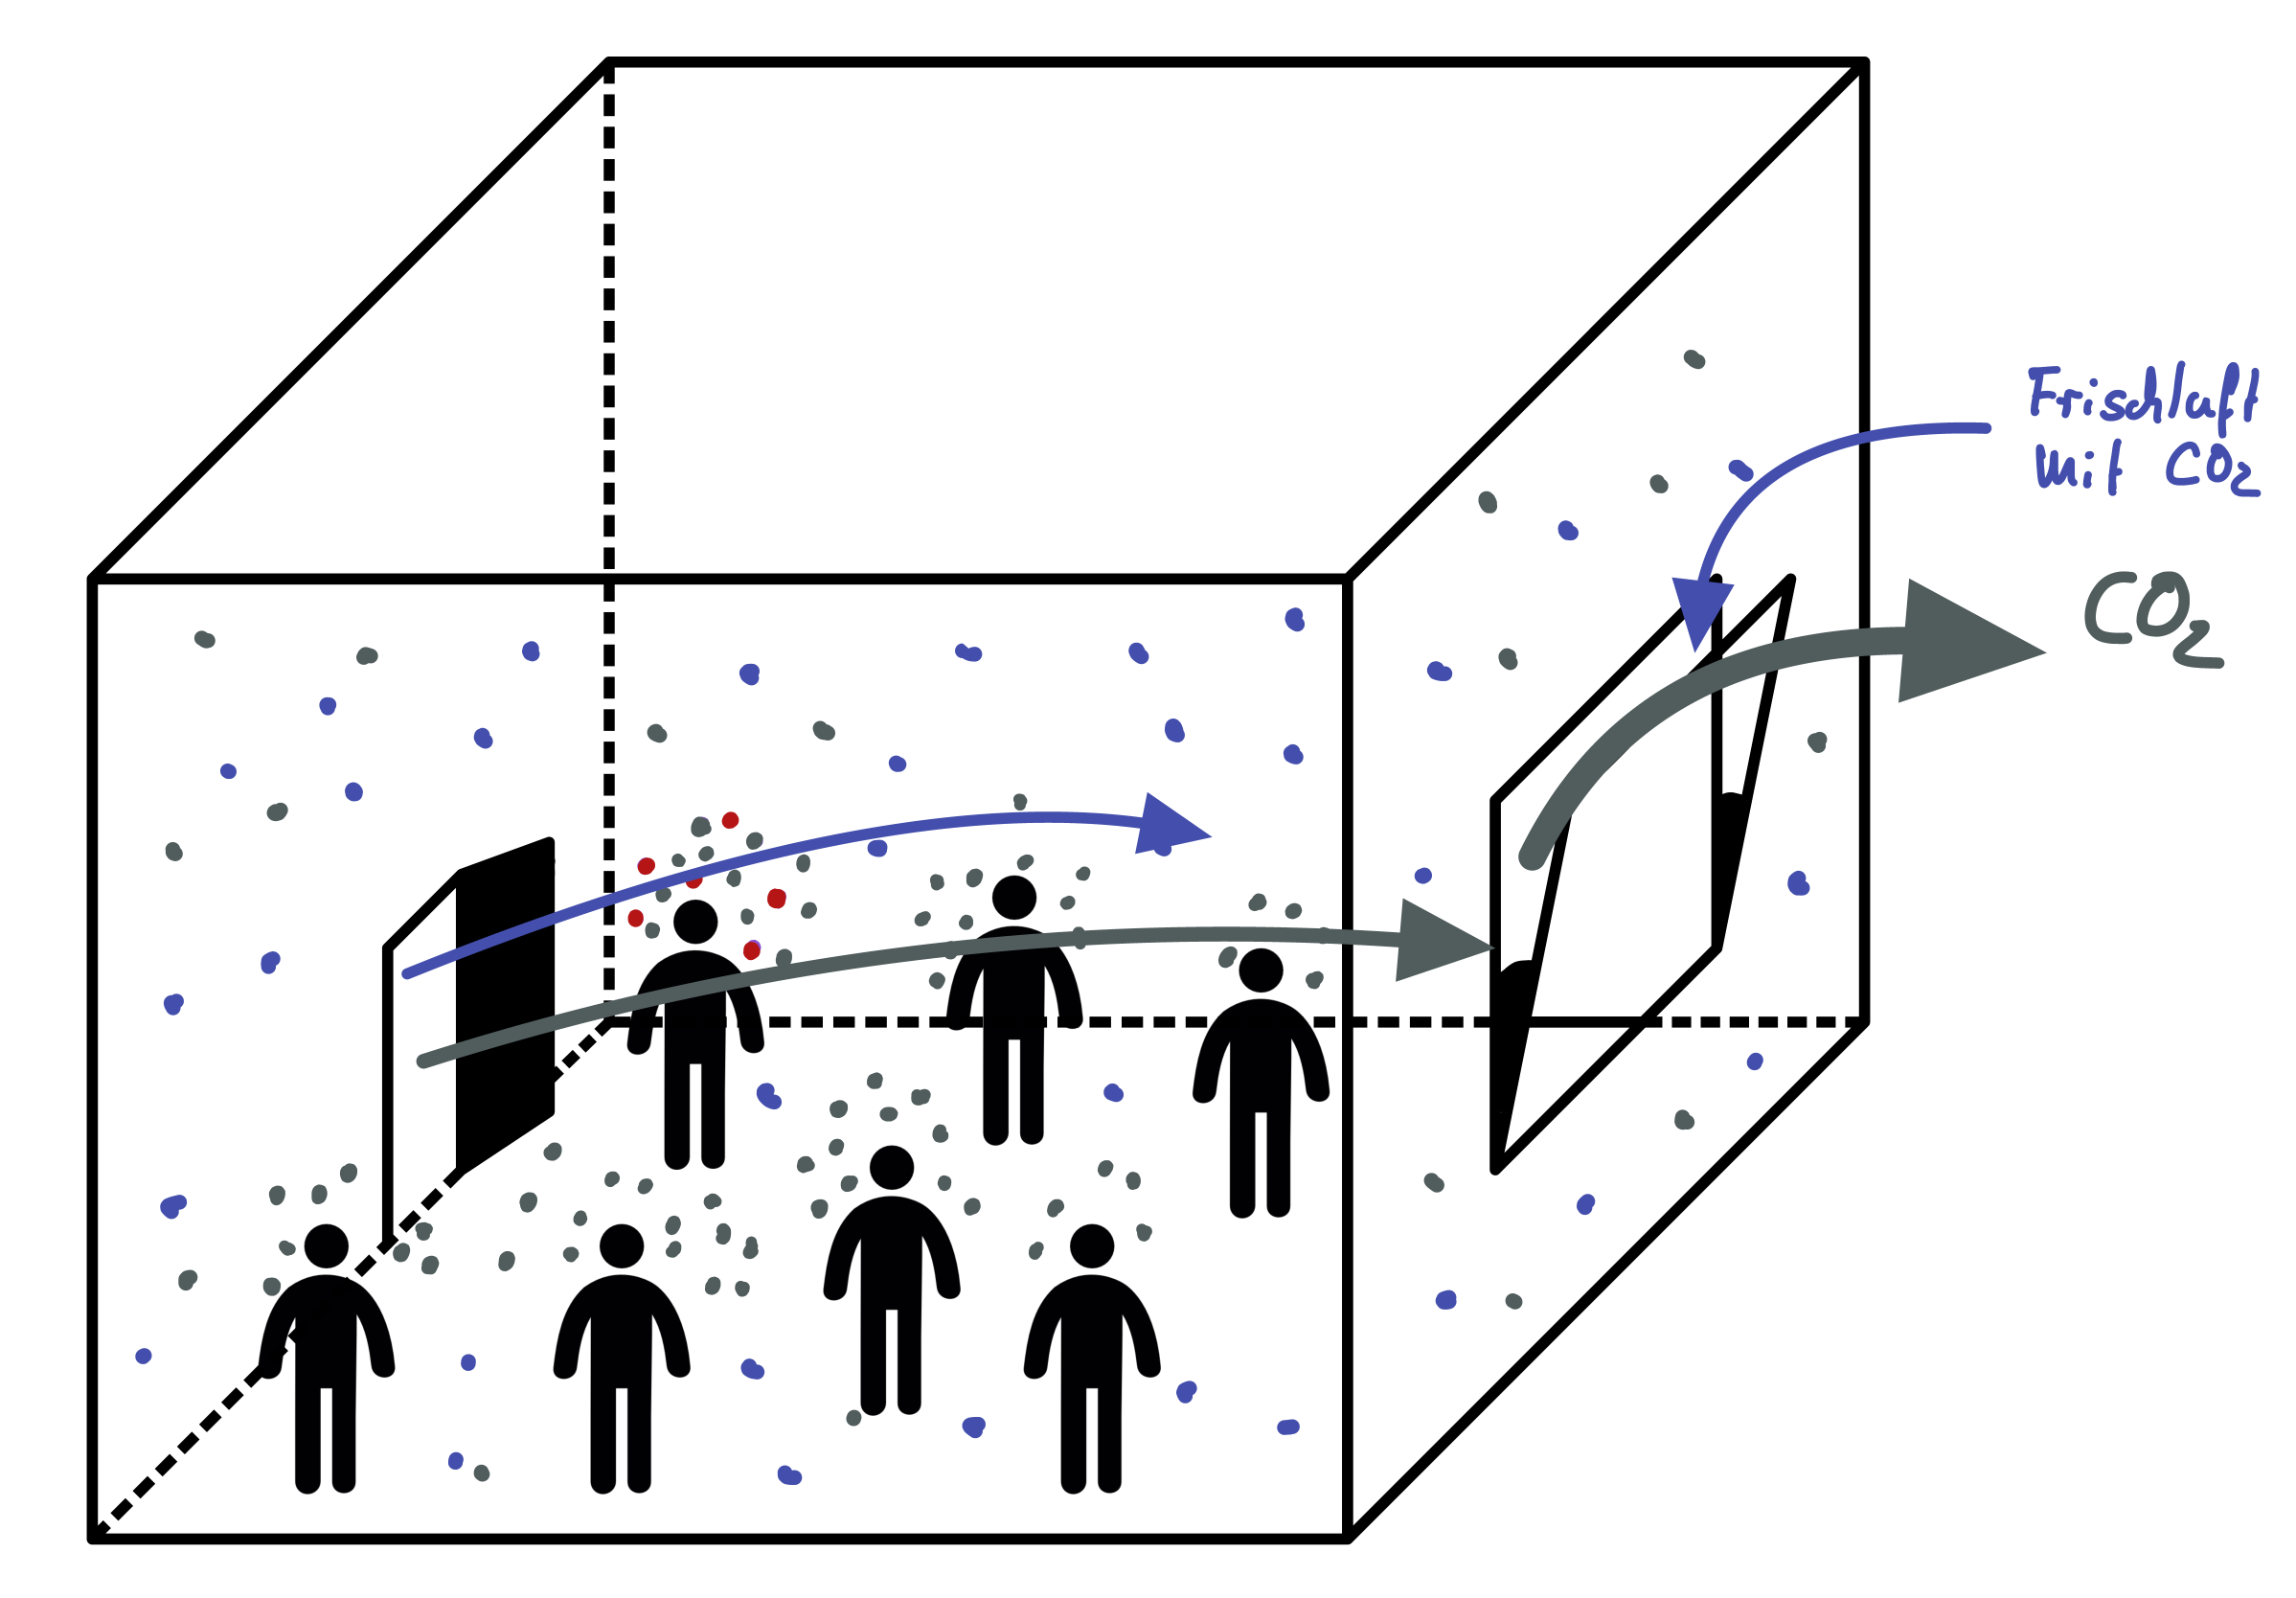
\includegraphics[width=1.\textwidth]{img/querluft}
	\end{minipage}
	\caption{Spaltluft- und Querluftströmung}
	\label{fig:querluft_spaltluft}
	\end{figure}
\FloatBarrier

\subsubsection*{Alkalisches Mauerwerk}
Auch das Mauerwerk kann für den \ce{CO2}-Gehalt entscheidend sein, da dabei der verarbeitete Kalkmörtel (bestehend aus Sand, Löschkalk und Kies) zu Calciumcarbonat reagiert. 
\begin{flalign*}
	\ce{Ca(OH)2 + CO2 -> CaCO3 + H2O}
\end{flalign*}

\newpage


\section{Rechnerisch den \ce{CO2}-Gehalt und die Luftwechselzahl bestimmen}

Um die \ce{CO2}-Konzentration mit bekannter Luftwechselzahl zu bestimmen ergibt sich mit der Hintergrundbelastung an \ce{CO2} aus der Umgebungsluft folgender Term:

\begin{flalign}
	\label{gl:co2}
	c_{\ce{CO2}} (t) &= c_{\ce{CO2}, \text{außen}} + \frac{N*\dot{V}_{\ce{CO2}}}{10*n*V}*\left[1-e^{-n*t}\right]
\end{flalign}

\begin{flalign}
	\label{gl:luftwechsel}
	n &= \frac{N*\dot{V}_{\ce{CO2}}}{10*V*\left[c_{\ce{CO2}}(t\rightarrow \infty)-c_{\ce{CO2},\text{außen}}\right]}
\end{flalign}

\begin{description}
	\item [$ \boldmath c_{\ce{CO2}} (t) \ldots$] Innenraum Konzentration an \ce{CO2} in Vol.\% zu einem \hspace{10mm} Zeitpunkt t
	\item [$\boldmath c_{\ce{CO2},\text{außen}}\ldots$] Außenkonzentration an \ce{CO2} in Vol.\% ($\approx $ 0,04 Vol.\%)
	\item [$ \boldmath c_{\ce{CO2}} (t\rightarrow \infty)\ldots$] Grenzkonzentration an \ce{CO2} für $t \rightarrow \infty$
	\item[$ \boldsymbol N\ldots$] Anzahl der Personen
	\item[$\boldsymbol n\ldots$] Luftwechselzahl in \si{\per \hour}
	\item[$\boldsymbol V\ldots$] Raumvolumen in \si{\kmeter}
	\item[$\boldmath \dot{V}_{\ce{CO2}}\ldots$] spezifische Emissionsrate in \si{\liter \per \hour}
	\item[$\boldsymbol t\ldots$] Zeit in \si{\hour}
\end{description}
\textit{Es gilt zu beachten, dass diese Gleichungen empirisch sind. So muss beachtet werden, dass die Gleichung nicht Einheiten gerecht ist und somit die Zahlenwerte der definierten Variablen zu nutzen sind !}

\subsection*{Herleitung der Gleichung für die \ce{CO2}-Konzentration}

Um die Gleichung \ref{gl:co2} herzuleiten, ist es nötig den Sachverhalt zu vereinfachen \mbox{(siehe Abb. \ref{fig:kompart})}. Die Blackbox stellt dabei den vereinfachten, betrachteten Raum dar in welchem der \ce{CO2}-Gehalt zum Zeitpunkt $t$ bestimmt werden soll.

\begin{figure}[h!]
	\centering
	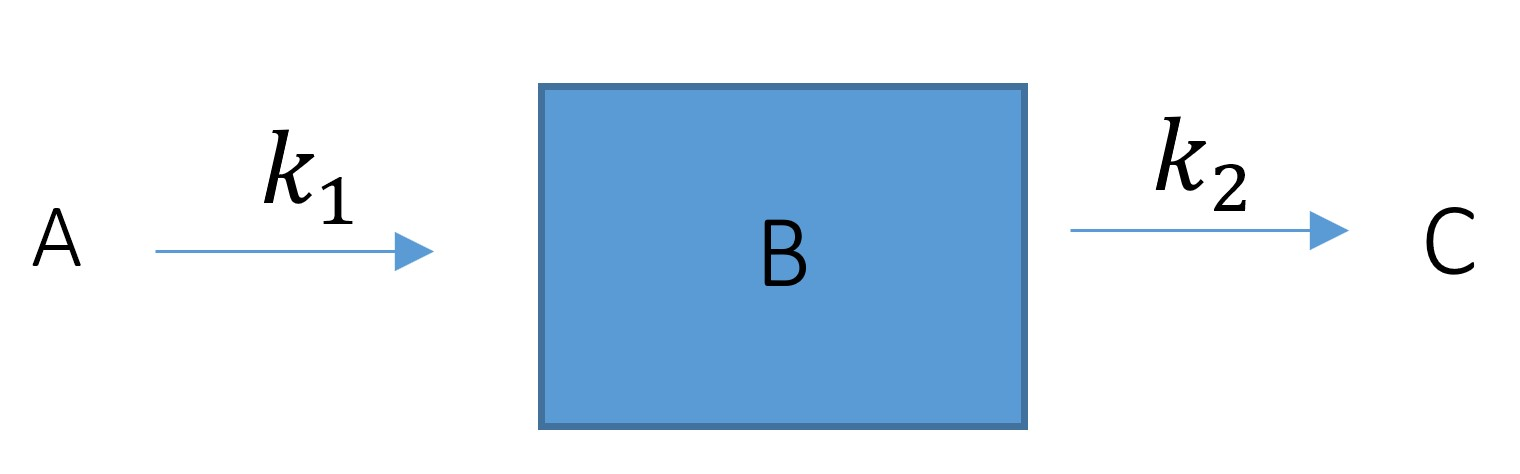
\includegraphics[width=0.8\textwidth]{img/kompart}
	\caption{"'Blackbox"'-Modell für \ce{CO2}-Gehalt eines Raumes}
	\label{fig:kompart}
\end{figure}
\FloatBarrier
%Ende
\begin{description}
	\item[$k_1\ldots$] Geschwindigkeitskonstante des eingehenden Stoffstromes A
	\item[$k_2\ldots$] Geschwindigkeitskonstante des ausgehenden Stoffstromes C
	\item[$A\ldots$] eingehender Stoffstrom A
	\item[$B\ldots$] "`Blackbox"' B
	\item[$C\ldots$]  ausgehender Stoffstrom C
	\item[$c_A\ldots$] Konzentration an \ce{CO2} des eingehenden Stoffstromes A
	\item[$c_B\ldots$] Konzentration an \ce{CO2} der "`Blackbox"' B
	\item[$c_C\ldots$]  Konzentration an \ce{CO2} des ausgehenden Stoffstromes C
\end{description}

Unter der Annahme, dass die Änderung der Konzentration an \ce{CO2} für die Stoffströme A und C konstant bleibt, kann ein differentieller Zusammenhang zwischen den Konzentrationen $c_A$ und $c_C$ jeweils mit der Zeit $t$ aufgestellt werden. Dieser Ausdruck ist unter de folgenden Gleichungen mit den Geschwindigkeitskonstanten $k_1$ und $k_2$ in einen Zusammenhang gebracht worden.
\begin{flalign}
	\dv{c_A}{t} &= - k_1 *c_A
\end{flalign}

\begin{flalign}
	\dv{c_c}{t} &= k_2 *c_B
\end{flalign}

Da A als eingehender Stoffstrom in der Blackbox "`verbraucht"' wird, erhält die Geschwindigkeitskonstante $k_1$ ein negatives Vorzeichen. Die Geschwindigkeitskonstante $k_2$ beschreibt den ausgehenden Stoffstrom , als würde dieser "`produziert"' und erhält somit ein positives Vorzeichen. Da der Stoffstrom C von der Konzentration in der Blackbox abhängig ist, wird hierbei mit der Konzentration $c_B$ gerechnet. Stoffstrom A ist lediglich vom \ce{CO2}-Gehalt außerhalb der Blackbox abhängig und ist somit lediglich abhängig von $c_A$.\\
Aus dem differentiellen Ansatz vom eingehenden Stoffstrom A und dem ausgehenden Stoffstrom B ergibt sich somit die Gleichung \ref{gl:cb}.
\begin{flalign}
	\label{gl:cb}
	\dv{c_B}{t} &= k_1*c_A-k_2*c_B
\end{flalign}
Die Vorzeichen ergeben sich erneut daraus ob die Stoffströme in die Blackbox eingetragen werden (+) oder die Blackbox verlassen (-).
Daraus lässt im folgenden die Gleichung für die \ce{CO2}-Konzentration aus bekannten Daten wie der Personenzahl $N$ oder der Luftwechselzahl $n$ berechnen.
\FloatBarrier

\vspace*{5mm}

\textbf{Umformungen für die Formel der \ce{CO2}-Konzentration in einem Raum in Abhängigkeit von der Zeit:}
\begin{flalign}
		c_b &= \frac{k_1}{k_2}*c_{A,0}*\left(1-e^{-k_2*t}\right)\\
			&= \frac{k_1}{k_2}*c_{A,0}*\left(1-e^{-k_2*t}\right)\\
			&= \frac{\frac{\dot{V}_{\ce{CO2}}}{V}}{k_2}*\frac{N}{10}*\left(1-e^{-k_2*t}\right)\\
			&= \frac{1}{k_2}*\frac{N*\dot{V}_{\ce{CO2}}}{10*V}*\left(1-e^{-k_2*t}\right)\\
	\tag{siehe Gl. \ref{gl:co2}}
	c_{\ce{CO2}, \text{innen}} (t) &= \frac{N*\dot{V}_{\ce{CO2}}}{10*n*V}*\left(1-e^{-n*t}\right) \\
	c_{\ce{CO2}} (t) &= c_{\ce{CO2}, \text{außen}} + \frac{N*\dot{V}_{\ce{CO2}}}{10*n*V}*\left[1-e^{-n*t}\right]	
\end{flalign}


\section{Beispielrechnungen}
Wie lassen sich diese Kenntnisse nun nutzen, um den \ce{CO2}-Gehalt zu bestimmen?

\subsection*{Beispiel 1:}
\textbf{Berechnung des \ce{CO2}-Gehaltes für eine bestimmte Personenzahl zu einem bestimmten Zeitpunkt t}\\

\textit{10 Studenten sind in einem Seminarraum $\left(V = \SI{150}{\kmeter}\right)$ mit gekippten Fenstern $\left(n = \SI{0,3}{\per \hour}\right)$ und es soll der \ce{CO2}-Gehalt nach \SI{1,5}{\hour} bestimmt werden. Da alle Personen sitzende Tätigkeiten ausführen kann von einer spezifischen Emissionsrate von \SI{17}{\liter\per\hour} an \ce{CO2} ausgegangen werden.}\\

\begin{minipage}[t]{0.45\textwidth}
	\textbf{Gegeben:}
	\begin{itemize}
		\item Personenzahl $N = 10$
		\item Luftwechselzahl $n = \SI{0,3}{\per \hour}$
		\item Raumvolumen $n = \SI{150}{\kmeter}$
		\item Zeit $t = \SI{1,5}{\hour}$
	\end{itemize}
\end{minipage}
\begin{minipage}[t]{0.5\textwidth}
	\textbf{}
	\begin{itemize}
		\item spezifische Emissionsrate $\dot{V}_{\ce{CO2}} = \SI{17}{\liter \per \hour} = \SI{17e-3}{\kmeter \per \hour}  $
		\item Außenkonzentration \ce{CO2} \\
		$c_{\ce{CO2}, \text{außen}} = \SI{4}{\volpercent}$
	\end{itemize}
\end{minipage}
\FloatBarrier

\vspace*{5mm}

\begin{minipage}[t]{0.7\textwidth}
	\textbf{Gesucht:}
	\begin{itemize}
		\item \ce{CO2}-Gehalt zum Zeitpunkt t
	\end{itemize}
\end{minipage}

\vspace*{5mm}

\textbf{Skizze:}
\begin{figure}[h!]
	\centering
	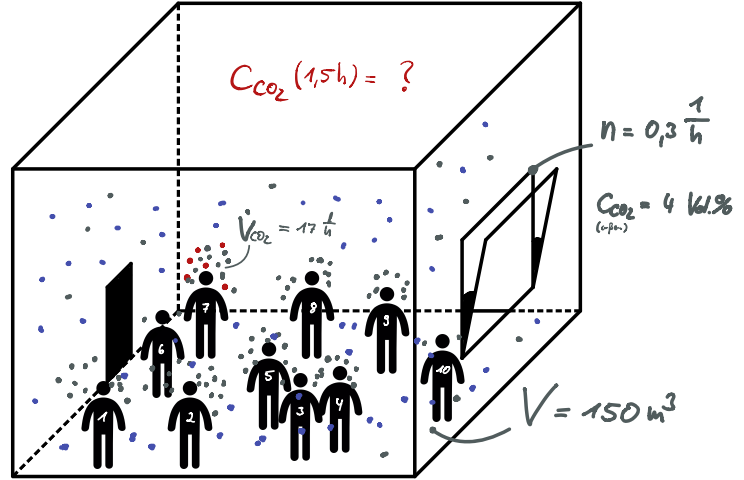
\includegraphics[width=0.5\textwidth]{img/beispiel 1}
	\caption{Skizze zu Beispiel 1}
	\label{fig:beispiel1}
\end{figure}
\FloatBarrier
%Ende

\newpage

\textbf{Lösung}:

\begin{flalign}
		\label{gl:beispiel1}
		c_{\ce{CO2}} (t) &= c_{\ce{CO2}, \text{außen}} + \frac{N*\dot{V}_{\ce{CO2}}}{10*n*V}*\left[1-e^{-n*t}\right]\\
		c_{\ce{CO2}} (\SI{1,5}{\hour}) &= \SI{0,04}{\volpercent} + \frac{10*\SI{17}{\liter\per \hour}}{10*\SI{0,3}{\per \hour}*\SI{150}{\kmeter}}*\left[1-e^{-\SI{0,3}{\per \hour}*\SI{1,5}{\hour}}\right]\\
						&= \SI{0,04}{\volpercent} +  \SI{0,137}{\volpercent}\\
						&= \underline{\SI{0,177}{\volpercent}}
\end{flalign}
\textit{Grenzkonzentration für DIN 1946 Teil II und \textsc{Pettenkofer}-Zahl überschritten!}

\subsection*{Beispiel 2:}
\textbf{Iterative Berechnung der Zeit t bis Grenzkonzentration erreicht ist}\\

\textit{Sieben Personen treffen sich zum studentischen Gelage in einer WG am Campus mit \SI{145}{\kmeter} Raumvolumen. Da ein halbgeöffnetes Fenster existiert, wird eine Luftwechselzahl von $n = \SI{0,26}{\per \hour}$ und durch den Milchgenuss eine Emissionsrate von \SI{25}{\liter \per \hour} gemessen. Die Außenkonzentration bleibt bei \SI{0,04}{\volpercent}. Es ist die Zeit zu bestimmen nach welcher eine Grenzkonzentration von \SI{0,15}{\volpercent} erreicht ist.}
\vspace*{5mm}

\begin{minipage}[t]{0.45\textwidth}
	\textbf{Gegeben:}
	\begin{itemize}
		\item Personenzahl $N = 7$
		\item Luftwechselzahl $n = \SI{1,05}{\per \hour}$
		\item Raumvolumen $n = \SI{145}{\kmeter}$
		\item Grenzkonzentration $c_{\ce{CO2}} = \SI{0,15}{\volpercent}$
	\end{itemize}
\end{minipage}
\begin{minipage}[t]{0.5\textwidth}
	\textbf{}
	\begin{itemize}
		\item spezifische Emissionsrate $\dot{V}_{\ce{CO2}} = \SI{25}{\liter \per \hour} $
		\item Außenkonzentration \ce{CO2} \\
		$c_{\ce{CO2}, \text{außen}} = \SI{4}{\volpercent}$
	\end{itemize}
\end{minipage}
\FloatBarrier

\vspace*{5mm}

\begin{minipage}[t]{1.0\textwidth}
	\textbf{Gesucht:}
	\begin{itemize}
		\item Zeitpunkt $t$ bis Grenzkonzentration erreicht ist
	\end{itemize}
\end{minipage}

\newpage

\textbf{Was ist iteratives Rechnen ?}\\
Iterationsverfahren beschreiben eine schrittweise Annäherung an eine Lösung durch wiederholte Ausführung einer Rechenvorschrift. Die Anzahl der Wiederholungen ist dabei abhängig von einer Abbruchbedingung, wie zum Beispiel die Genauigkeit der Nachkommastellen des Ergebnisses.\\
Sinnvoll ist diese Art Berechnung wenn nicht genügend Informationen über Parameter vorliegen oder sich ein umstellen der Gleichung nach einem bestimmten Parameter, als zu komplex erweist. \\
In der verfahrenstechnischen Praxis findet sich das iterative Rechnen im Excel-Add-In \textit{Solver} wieder. Auch dieses Add-In rechnet mit der iterativen Methodik.

%\vspace{-5mm}
\begin{center}
	\begin{figure}[h!]
		\centering
		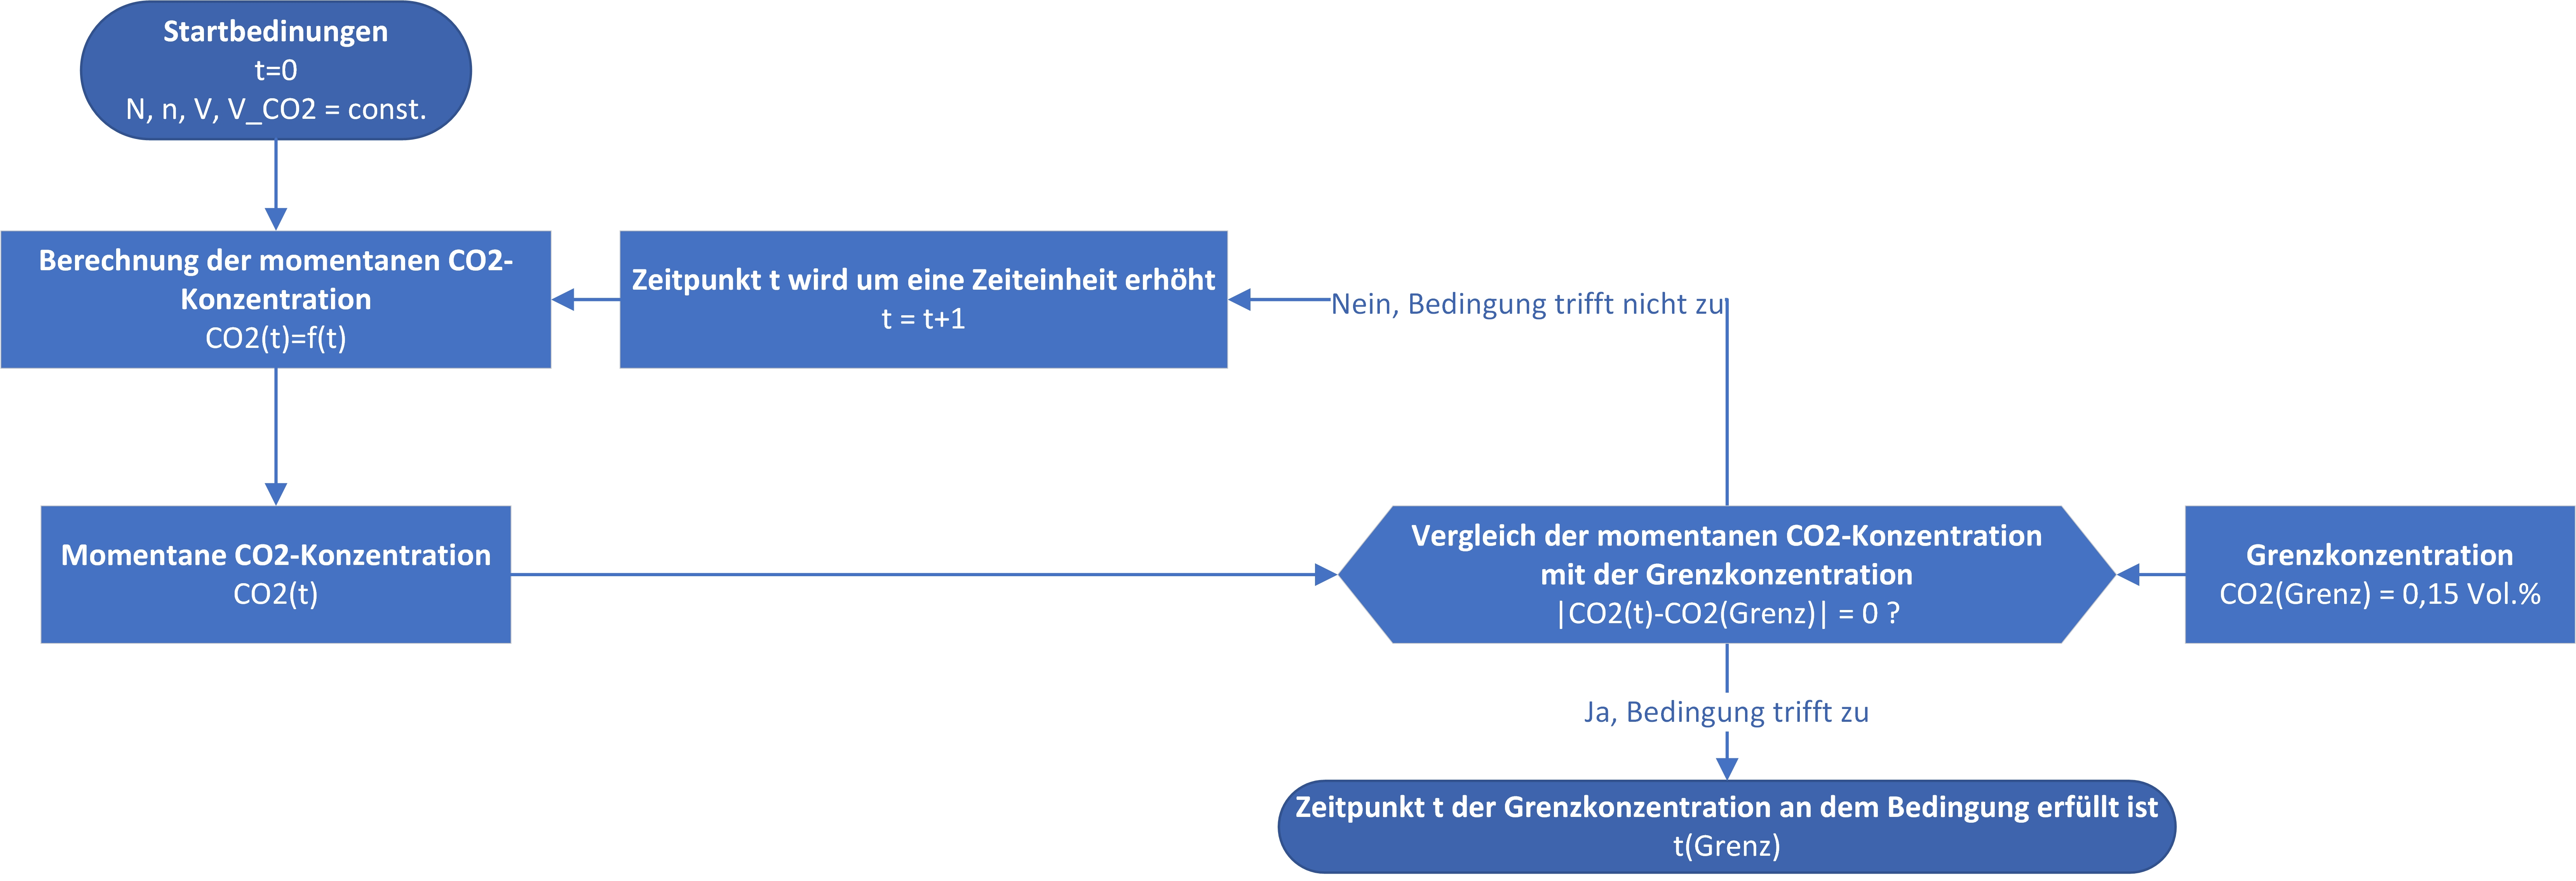
\includegraphics[width=1.1\textwidth]{img/iterativ}
		\caption{Übersicht zum iterativen Rechnen der \ce{CO2}-Konzentration}
\end{figure}
\end{center}

\FloatBarrier
%Ende

\newpage

\textbf{Lösung:}
\begin{enumerate}
	\item \textbf{Durchlauf} für $t = \SI{0}{\hour}$:\\
	\begin{flalign}
		c_{\ce{CO2}} (\SI{0}{\hour}) &= \SI{0,04}{\volpercent} + \frac{10*\SI{25}{\liter\per \hour}}{10*\SI{1,05}{\per \hour}*\SI{145}{\kmeter}}*\left[1-e^{-\SI{1,05}{\per \hour}*\SI{0}{\hour}}\right]\\
		&= \SI{0,040}{\volpercent}\\
		\Delta c_{\ce{CO2}} &= \abs{c_{\ce{CO2}}-c_{\text{Grenz}}}\\
													&=\abs{\SI{0,040}{\volpercent}-\SI{0,150}{\volpercent}}\\
													&= \SI{0,110}{\volpercent} > 0 \rightarrow \text{Wiederholung mit } t+1
	\end{flalign}
\item \textbf{Durchlauf} für $t = \SI{1}{\hour}$:\\
\begin{flalign}
	c_{\ce{CO2}} (\SI{1}{\hour}) &= \SI{0,04}{\volpercent} + \frac{10*\SI{25}{\liter\per \hour}}{10*\SI{1,05}{\per \hour}*\SI{145}{\kmeter}}*\left[1-e^{-\SI{1,05}{\per \hour}*\SI{1}{\hour}}\right]\\
	&= \SI{0,115}{\volpercent}\\
	\Delta c_{\ce{CO2}} &= \abs{\SI{0,115}{\volpercent}-\SI{0,150}{\volpercent}}\\
	&= \SI{0,035}{\volpercent} > 0 \rightarrow \text{Wiederholung mit } t+1
\end{flalign}
\item \textbf{Durchlauf} für $t = \SI{2}{\hour}$:\\
\begin{flalign}
	c_{\ce{CO2}} (\SI{2}{\hour}) &= \SI{0,04}{\volpercent} + \frac{10*\SI{25}{\liter\per \hour}}{10*\SI{1,05}{\per \hour}*\SI{145}{\kmeter}}*\left[1-e^{-\SI{1,05}{\per \hour}*\SI{2}{\hour}}\right]\\
	&= \SI{0,141}{\volpercent}\\
	\Delta c_{\ce{CO2}} &= \abs{\SI{0,141}{\volpercent}-\SI{0,150}{\volpercent}}\\
	&= \SI{0,009}{\volpercent} > 0 \rightarrow \text{Wiederholung mit } t+1
\end{flalign}
\item \textbf{Durchlauf} für $t = \SI{3}{\hour}$:\\
\begin{flalign}
	c_{\ce{CO2}} (\SI{3}{\hour}) &= \SI{0,04}{\volpercent} + \frac{10*\SI{25}{\liter\per \hour}}{10*\SI{1,05}{\per \hour}*\SI{145}{\kmeter}}*\left[1-e^{-\SI{1,05}{\per \hour}*\SI{3}{\hour}}\right]\\
	&= \SI{0,150}{\volpercent}\\
	\Delta c_{\ce{CO2}} &= \abs{\SI{0,150}{\volpercent}-\SI{0,150}{\volpercent}}\\
	&= \SI{0,000}{\volpercent} = 0 \rightarrow \text{Zeit der Grenzkonzentration}
\end{flalign}
\end{enumerate}

\newpage

\subsection*{Beispiel 3:}
\textbf{Einfluss der Personenzahl auf den Verlauf der \ce{CO2}-Konzentration}\\

\textit{Es soll der Verlauf der Konzentration an \ce{CO2} in Abhängigkeit von einer, 10 und 20 Personen grafisch dargestellt werden. Der Raum hat ein Volumen von \SI{145}{\kmeter} und es ist von einer Luftwechselzahl von \SI{1,05}{\per \hour} auszugehen. Es wurde eine Außenkonzentration von \SI{0,04}{\volpercent}, sowie eine spezifischen Emissionsrate von \SI{25}{\liter\per\hour} an \ce{CO2}.}

% Table generated by Excel2LaTeX from sheet 'Tabelle1'
\begin{table}[h!]
	\renewcommand*{\arraystretch}{1.2}
	\centering
	\rowcolors{2}{white}{gray!25}
	\caption{Daten für \ce{CO2}-Konzentration für verschiedenen Personenzahlen}
	\resizebox{\textwidth}{!}{
	\begin{tabulary}{1.0\textwidth}{c|ccc|cc}
		\hline
		Zeit [h]&c [Vol.\%] für 1 Pers. & c [Vol.\%] für 10 Pers.& c [Vol.\%] für 20 Pers. & \textsc{Pettenkofer}-Zahl & DIN 1946 Teil 2 \\
		\hline
		0,00  & 0,040 & 0,040 & 0,040 & 0,10   & 0,15 \\
		0,25  & 0,059 & 0,078 & 0,116 & 0,10   & 0,15 \\
		0,50  & 0,074 & 0,107 & 0,174 & 0,10   & 0,15 \\
		0,75  & 0,085 & 0,129 & 0,219 & 0,10   & 0,15 \\
		1,00  & 0,093 & 0,147 & 0,253 & 0,10   & 0,15 \\
		1,25  & 0,100 & 0,160 & 0,280 & 0,10   & 0,15 \\
		1,50  & 0,105 & 0,170 & 0,300 & 0,10   & 0,15 \\
		1,75  & 0,109 & 0,178 & 0,316 & 0,10   & 0,15 \\
		2,00  & 0,112 & 0,184 & 0,328 & 0,10   & 0,15 \\
	\end{tabulary}%
	\label{tab:tabelle_co2}%
}
\end{table}%


\begin{figure}[h!]
	\begin{center}
		\resizebox{0.75\textwidth}{!}{
			\begin{tikzpicture}[trim axis left, trim axis right]
				\begin{axis}[
					grid =both,
					axis lines = left,
					width = 15cm,
					height = 8cm,
					xmin = 0,
					xmax = 2.,
					ymin = 0,
					ymax = 0.4,
					ytick = {0,0.04,0.1,0.15,...,0.4},
					%xtick = {0,1,...,5},
					ylabel={\ce{CO2}-Konzentration in \si{\volpercent}},
					%y label style={at={(0,0.5)}},
					xlabel={Zeit in \si{\hour}},
					legend style={at={(1.05,0.75)},anchor=west},
					%	y dir = reverse,
					yticklabel style={/pgf/number format/fixed},
					]
					
					%1 Person
					\addplot [color=black, mark=*] coordinates{(0,0.04) (0.25,5.89551424984753E-02) (0.5,7.35340423344158E-02) (0.75,8.47470585617263E-02) (1,9.33712849662434E-02) (1.25,0.100004404866241) (1.5,0.105106112259347) (1.75,0.109029969918679) (2,0.112047912294501)};
					
					%10 Person
					\addplot [color=blue, mark=*] coordinates{(0,0.04) (0.25,7.79102849969507E-02) (0.5,0.107068084668832) (0.75,0.129494117123453) (1,0.146742569932487) (1.25,0.160008809732482) (1.5,0.170212224518694) (1.75,0.178059939837358) (2,0.184095824589001)};
					
					%20 Person
					\addplot [color=red, mark=*] coordinates{(0,0.04) (0.25,0.115820569993901) (0.5,0.174136169337663) (0.75,0.218988234246905) (1,0.253485139864974) (1.25,0.280017619464964) (1.5,0.300424449037388) (1.75,0.316119879674716) (2,0.328191649178003) };
					
					\addplot[mark=none, black, dotted, samples=2] {0.1};
					\addplot[mark=none, black, dashed, samples=2] {0.15};
				 
				 	\legend{1 Person, 10 Personen, 20 Personen, \textsc{Pettenkofer}-Zahl, DIN 1946 Teil 2}
				\end{axis}
			\end{tikzpicture}
		}
		\caption{Verlauf der gemittelten Temperaturdifferenzen}
		\label{dia:tdiffverlauf}
	\end{center}
\end{figure}
\FloatBarrier

\section{Aufgaben zur \ce{CO2}-Konzentration in Räumen}
\subsubsection*{Wie oft sollte nun gelüftet werden, um einer Verbreitung von Aerosolen vorzubeugen?}

\subsection*{Aufgaben:}
In einem Seminarraum $(V=\SI{200}{\kmeter})$ befinden sich 30 Studenten. Sie führen sitzende Tätigkeiten aus mit einer \ce{CO2}-Abgabe von \SI{15}{\liter \per \hour}. Laut DGUV, der deutschen gesetzlichen Unfallversicherung, soll nach der folgenden Tabelle regelmäßig gelüftet werden. Die \ce{CO2}-Konzentration in der Atmosphäre ist mit 0,04 Vol.\% anzunehmen. Die Luftfeuchtigkeit wird nicht berücksichtigt.

\begin{table}[h!]
	\renewcommand*{\arraystretch}{1.2}
	\centering
	\rowcolors{2}{white}{gray!25}
	\caption{Regelmäßiges Lüften zur Sicherheit vor Corona \cite{e.V..2020}}
	\label{tab:corona_lueften}
	\begin{tabulary}{1.0\textwidth}{C|C|C}
		\hline
		& \textbf{Winter} &\textbf{Sommer}\\
		\textbf{Büroräume}	& in \SI{1}{\hour} für \SI{3}{\minute} lüften&in \SI{1}{\hour} für \SI{10}{\minute} lüften\\
		\textbf{Seminarräume} & in \SI{20}{\minute} für \SI{3}{\minute} lüften & in \SI{20}{\minute} für \SI{10}{\minute} lüften\\
		\hline			
	\end{tabulary}
\end{table}
\FloatBarrier

\begin{enumerate}
	\item [a)] 	Welche Konzentration an \ce{CO2} (ppm) liegt nach 1,5 h Vorlesung vor, wenn der Raum mit einer Luftwechselzahl von n=0,1 kaum gelüftet wird?{\scriptsize  (3530 ppm)}
	
	\item [b)] Nach dem letzten Block wird der Seminarraum gewechselt und einige Studenten sind bereits nach Hause gegangen. Im neuen Seminarraum $\SI{146}{\kmeter}$ befinden sich nun nur noch 21 Studenten. In diesem Raum soll die \textsc{Pettenkofer}-Zahl nicht überschritten werden. Durch das Wechseln des Raumes geben die Studenten für die 45 min Seminar nun \SI{18}{\liter \per \hour}  \ce{CO2 } ab. 
	Wie hoch muss die Luftwechselzahl sein, um den geforderten Grenzwert einzuhalten? {\scriptsize (\SI{3,89}{\per \hour})}
	
	\item [c)] Welche Luftwechselzahl ergibt sich für 15 Studenten im Raum aus 1 a), wenn es Winter ist und die nötige Regelmäßigkeit der Lüftung zur Sicherheit vor Aerosolbildung einzuhalten ist? Reicht dieser Luftwechselzahl um den Grenzwert der DIN 1946-2 oder der Pettenkofer-Zahl einzuhalten?\\
	Es wird davon ausgegangen, dass mit den Fenstern stoßgelüftet wird und entweder alle Fenster und Türen offen oder zu sind.\\
	{\scriptsize (reicht nicht für Pettenkofer oder DIN 1946-2, \SI{0,32}{\per \hour} < \SI{0,62}{\per \hour}< \SI{1,74}{\per \hour})}
	
	\item [d)] Werden die Grenzwerte im Sommer eingehalten? 
	{\scriptsize (reicht nicht für Pettenkofer, aber für DIN 1946-2, \SI{0,62}{\per \hour}< \SI{1,08}{\per \hour} < \SI{1,74}{\per \hour})}
	
	\item [e)] Wie lang muss im Winter und im Sommer für c) und d) pro 20 min gelüftet werden um die Grenzwerte für \textsc{Pettenkofer} und DIN 1946-2 einzuhalten?
	{\scriptsize (Sommer/Winter: DIN mind. alle 20 min 5,8 min lüften, Pettenkofer mind. alle 20 min 16,2 min lüften)}
		
\end{enumerate}

%Praktikumsskript, Modul ………, Versuch …….., Prof. Musterprof. 
%DIN 12345, Jahr der Veröffentlichung 
%Link der Internetseite, Zugriffsdatum 
%Buchtitel, Autor, Verlag, Veröffentlichungsjahr 

%Literaturverzeichnis Bücher
\bibliography{Literatur}
\bibliographystyle{unsrtdin}
\addcontentsline{toc}{section}{Literaturverzeichnis}



\section*{Anhang}
\addcontentsline{toc}{section}{Anhang}
\label{sec:anhang}

%Betriebsanweisung

%\include{09_erklaerung}

\end{document}
